\section{System Design}
\label{sec:system_design}
\subsection{Embedded system architecture}
As a hardware/software co-design, the system architecture is an embedded CPU+FPGA-based platform, where the acceleration of Conv2D and DepthwiseConv2D tensor operations. \fig{fig:hw_sbs} illustrates the system \replaced{hardware architecture}{overview} as a scalable structure. For \REVIEW{hyperparameter} configuration, each PU uses AXI-Lite interface. For data transfer, each PU uses AXI-Stream interfaces via Direct Memory Access (DMA) allowing data movement with high transfer rate. Each PU asserts an interrupt flag once the job or transaction is complete. This interrupt event is handled by the embedded CPU to collect results and start a new transaction.

The hardware architecture can resize its resource utilization by changing the number of PUs instances \REVIEW{prior to the hardware synthesis}, this provides scalability with a good trade-off between area and throughput. The dedicated PUs for \emph{Conv} and \emph{FC} implement the proposed dot-product approximation as a system component. The PUs are written in C using Vivado HLS (High-Level Synthesis) tool. In this publication, we illustrate the integration of the approximate dot-product component on the \emph{Conv} processing unit.


The embedded system architecture is implemented on Xilinx Zynq devices. In this paper, we present a use case with Zynq-7020.  processing system (PS), we use a single CPU core ARM Cortex-A9 with NEON floating point unit (FPU) running at 666MHz. The proposed hardware accelerator is  the CPU though AXI-Lite interface, and connected with a direct memory access (DMA) t the high-performance to an off-chip memory RAM with 1 GB. communication

Regarding the software architecture, this is structured as a
layered object-oriented application framework written in the C programming language. This offers a comprehensive high level embedded software application programming interface (API) that allows the construction of scalable sequential SbS networks with configurable hardware acceleration. Conceptually this design is modular, reusable, and extensible. The overall structure is depicted in \fig{fig:sw_stack}.


In this section, we exploit the hybrid custom floating-point and logarithmic dot-product approximation presented in \cite{nevarez2021accelerating}.


\begin{figure}[t!]
	\centering
	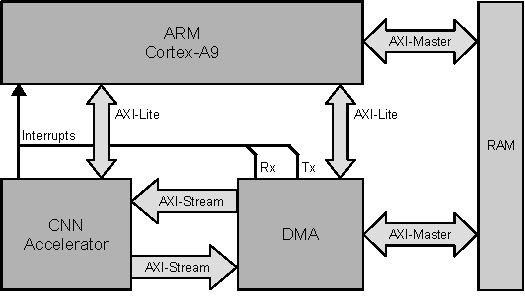
\includegraphics[width=0.5\textwidth]{../figures/system_design.pdf}
	\caption{System-level architecture of the proposed embedded platform.}
	\label{fig:system_architecture}
\end{figure}

\begin{figure}[t!]
	\centering
	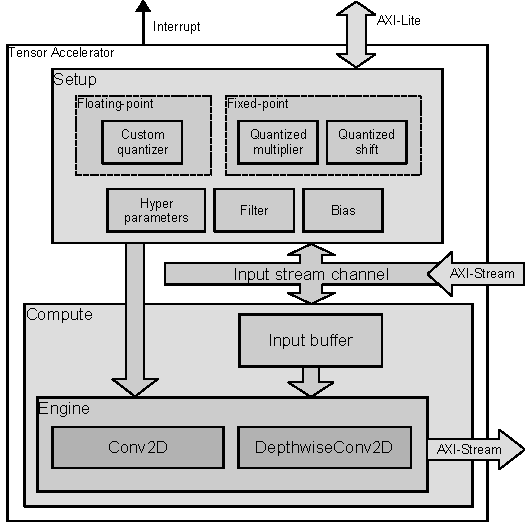
\includegraphics[width=0.5\textwidth]{../figures/accelerator.pdf}
	\caption{Hardware architecture of the proposed accelerator.}
	\label{fig:accelerator}
\end{figure}

\begin{figure}[t!]
	\centering
	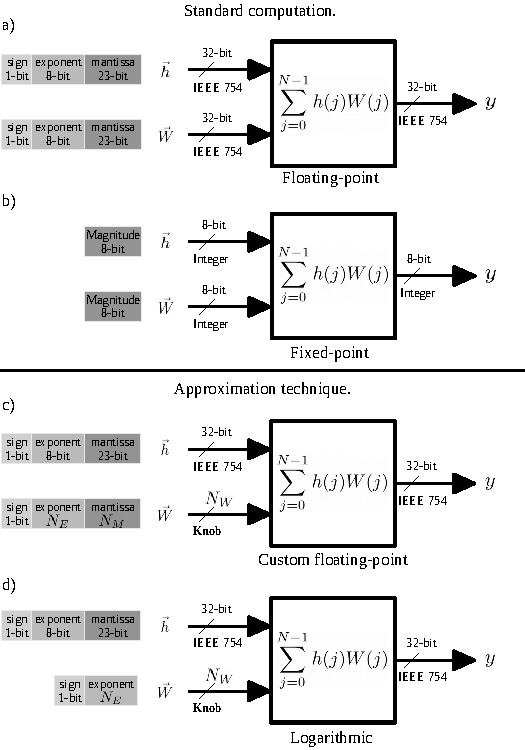
\includegraphics[width=0.5\textwidth]{../figures/dot-product_unit.pdf}
	\caption{Proposed hardware modules for vector dot-product.}
	\label{fig:dot_product}
\end{figure}

\begin{figure}[t!]
	\centering
	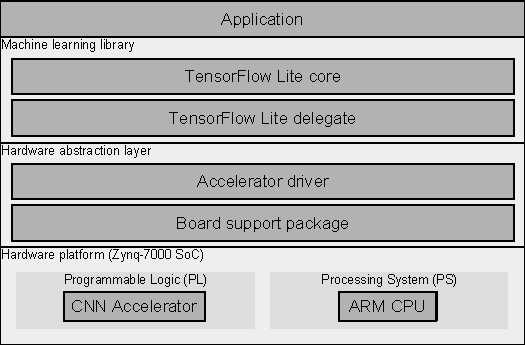
\includegraphics[width=0.5\textwidth]{../figures/sw_stack.pdf}
	\caption{System-level overview of the embedded software architecture.}
	\label{fig:sw_stack}
\end{figure}

